\documentclass{article}
\usepackage{url}
\usepackage[english]{babel}
\usepackage[utf8]{inputenc}
\usepackage{color}
\usepackage{graphicx}


\title{Milestone 2}
\author{Mirosław Kuźniar, Szymon Porzeziński, Bartosz Skrzypczak }
\date{\today}

\begin{document}

\maketitle

\section{Description}
The main goal of this project is to run a simulation of liftoff and flight of a rocket. The rocket will be composed of sub-assemblies, such as an engine and a fuel container. Parameters of these components and external factors will have an influence on the final result of the simulation. The whole process will be considered as completed when the rocket reaches a given attitude or comes back to the ground. 

\section{Noun-verb method}
The \textcolor{blue}{simulated world} will contain the \textcolor{blue}{rocket} and have \textcolor{blue}{force fields}, representing different extrenal forces acting on the rocket. The world will need a way to \textcolor{yellow}{run the simulation}. A \textcolor{blue}{rocket} will contain multiple \textcolor{blue}{rocket parts}, with attributes that may affect the course of the simulation. Each component will have \textcolor{blue}{mass} and will be able to \textcolor{yellow}{create thrust force}, which can depend on it's rotation. The \textcolor{blue}{engine} will \textcolor{yellow}{create thrust force} based on a \textcolor{blue}{thrust curve} provided by the user and the \textcolor{blue}{amount of remaining fuel} in the \textcolor{blue}{fuel tank}. The movement of the \textcolor{blue}{rocket} will depend on the \textcolor{blue}{force of gravity}, \textcolor{blue}{wind} and \textcolor{blue}{air resistance}. The world simulation will also \textcolor{yellow}{check whether the rocket has reached a given attitude or returned to the ground}, and stop the simulation.

\section{Use case diagram}
\hspace{-70pt}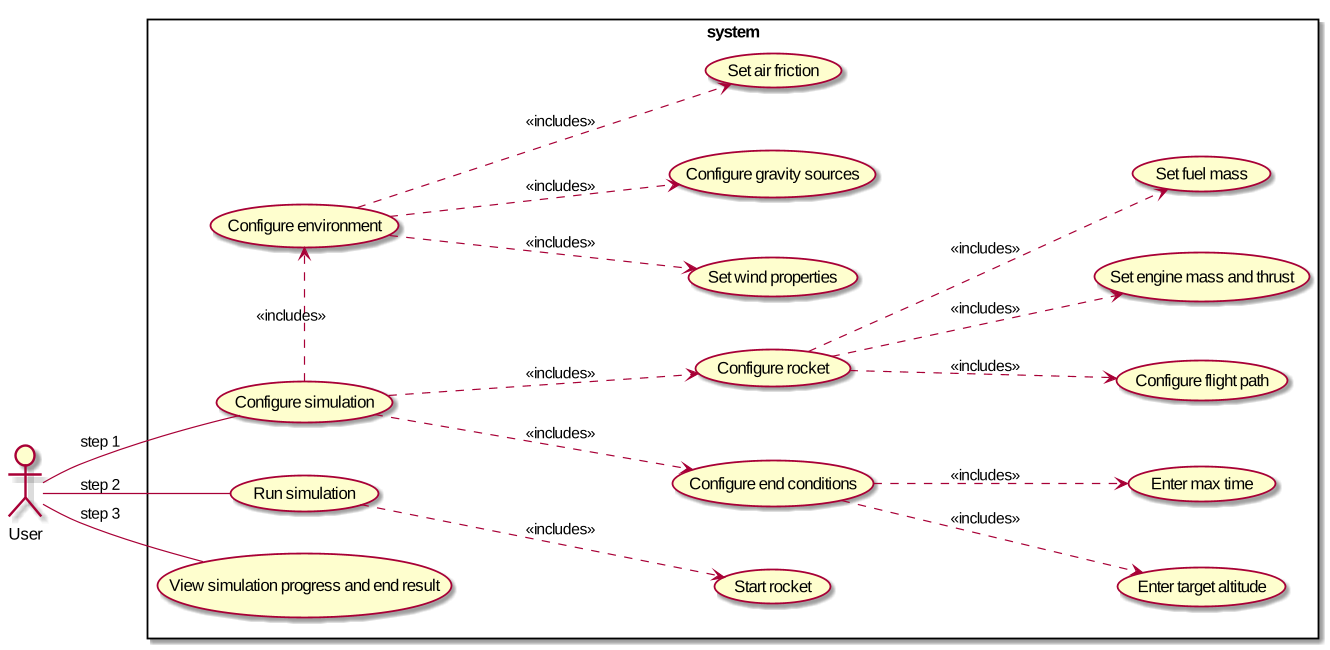
\includegraphics[width=17cm]{use_case_diagram.png}
\vspace{5cm}
\section{CRC cards}

\begin {center}

\begin{tabular}{|c|c|}
\hline
\multicolumn{2}{|l|}{\textbf{Classname:} Rocket}\\
\hline
\multicolumn{2}{|l|}{\textbf{Superclass:} none}\\
\multicolumn{2}{|l|}{\textbf{Subclass/es:} none}\\
\hline
\parbox[]{5cm}{\vspace{3px}\textbf{Responsibilities:} \\Coordinates interactions between its parts, and stores the current state of the rocket (position, velocity, direction)\vspace{3px}} & \parbox[]{5cm}{\textbf{Collaborations:}\\Engine\\Tank\\Vector}\\
\hline
 \end{tabular}\vspace{.4cm}
 
\begin{tabular}{|c|c|}
\hline
\multicolumn{2}{|l|}{\textbf{Classname:} Engine}\\
\hline
\multicolumn{2}{|l|}{\textbf{Superclass:} IRocketPart}\\
\multicolumn{2}{|l|}{\textbf{Subclass/es:} none}\\
\hline
\parbox[]{5cm}{\vspace{3px}\textbf{Responsibilities:} \\Based on its own thrust values and the amount of remaining fuel, creates thrust force\vspace{3px}} & \parbox[]{5cm}{\textbf{Collaborations:}\\FuelTank\\Vector}\\
\hline
 \end{tabular}\vspace{.4cm}

\begin{tabular}{|c|c|}
\hline
\multicolumn{2}{|l|}{\textbf{Classname:} Tank}\\
\hline
\multicolumn{2}{|l|}{\textbf{Superclass:} IRocketPart}\\
\multicolumn{2}{|l|}{\textbf{Subclass/es:} none}\\
\hline
\parbox[]{5cm}{\vspace{3px}\textbf{Responsibilities:} \\Keeps track of the amount (mass) of the remaining fuel\vspace{3px}} & \parbox[]{5cm}{\textbf{Collaborations:}\\none}\\
\hline
 \end{tabular}\vspace{.4cm}

\begin{tabular}{|c|c|}
\hline
\multicolumn{2}{|l|}{\textbf{Classname:} Wind}\\
\hline
\multicolumn{2}{|l|}{\textbf{Superclass:} IForceField}\\
\multicolumn{2}{|l|}{\textbf{Subclass/es:} none}\\
\hline
\parbox[]{5cm}{\vspace{3px}\textbf{Responsibilities:} \\Creates a force based on wind speed and direction at a given point\vspace{3px}} & \parbox[]{5cm}{\textbf{Collaborations:}\\Vector}\\
\hline
 \end{tabular}\vspace{.4cm}

\begin{tabular}{|c|c|}
\hline
\multicolumn{2}{|l|}{\textbf{Classname:} GravityField}\\
\hline
\multicolumn{2}{|l|}{\textbf{Superclass:} IForceField}\\
\multicolumn{2}{|l|}{\textbf{Subclass/es:} none}\\
\hline
\parbox[]{5cm}{\vspace{3px}\textbf{Responsibilities:} \\Calculates the force of gravity, based on position\vspace{3px}} & \parbox[]{5cm}{\textbf{Collaborations:}\\Vector}\\
\hline
 \end{tabular}\vspace{.4cm}

\begin{tabular}{|c|c|}
\hline
\multicolumn{2}{|l|}{\textbf{Classname:} AirResistanceField}\\
\hline
\multicolumn{2}{|l|}{\textbf{Superclass:} IForceField}\\
\multicolumn{2}{|l|}{\textbf{Subclass/es:} none}\\
\hline
\parbox[]{5cm}{\vspace{3px}\textbf{Responsibilities:} \\Calculates the force of air resistance, based on position and speed\vspace{3px}} & \parbox[]{5cm}{\textbf{Collaborations:}\\Vector}\\
\hline
 \end{tabular}\vspace{.4cm}

\begin{tabular}{|c|c|}
\hline
\multicolumn{2}{|l|}{\textbf{Classname:} IForceField}\\
\hline
\multicolumn{2}{|l|}{\textbf{Superclass:} none}\\
\multicolumn{2}{|l|}{\textbf{Subclass/es:} Wind, GravityField, AirResistanceField}\\
\hline
\parbox[]{5cm}{\vspace{3px}\textbf{Responsibilities:} \\A general interface for interacting with force fields\vspace{3px}} & \parbox[]{5cm}{\textbf{Collaborations:}\\Vector}\\
\hline
 \end{tabular}\vspace{.4cm}

\begin{tabular}{|c|c|}
\hline
\multicolumn{2}{|l|}{\textbf{Classname:} Vector}\\
\hline
\multicolumn{2}{|l|}{\textbf{Superclass:} none}\\
\multicolumn{2}{|l|}{\textbf{Subclass/es:} none}\\
\hline
\parbox[]{5cm}{\vspace{3px}\textbf{Responsibilities:} \\Storage and operations on vectors\vspace{3px}} & \parbox[]{5cm}{\textbf{Collaborations:}\\none}\\
\hline
 \end{tabular}\vspace{.4cm}

\begin{tabular}{|c|c|}
\hline
\multicolumn{2}{|l|}{\textbf{Classname:} IRocketPart}\\
\hline
\multicolumn{2}{|l|}{\textbf{Superclass:} none}\\
\multicolumn{2}{|l|}{\textbf{Subclass/es:} Engine, Tank}\\
\hline
\parbox[]{5cm}{\vspace{3px}\textbf{Responsibilities:} \\Can have mass and may be a source of a force\vspace{3px}} & \parbox[]{5cm}{\textbf{Collaborations:}\\Vector}\\
\hline
 \end{tabular}\vspace{.4cm}

\begin{tabular}{|c|c|}
\hline
\multicolumn{2}{|l|}{\textbf{Classname:} World}\\
\hline
\multicolumn{2}{|l|}{\textbf{Superclass:} none}\\
\multicolumn{2}{|l|}{\textbf{Subclass/es:} none}\\
\hline
\parbox[]{5cm}{\vspace{3px}\textbf{Responsibilities:} \\Controls the simulation, determines when to start and stop it, and shows the results\vspace{3px}} & \parbox[]{5cm}{\textbf{Collaborations:}\\Rocket\\IForceField}\\
\hline
 \end{tabular}\vspace{.4cm}

\end{center}

\section{UML Class Diagrams}
\hspace{-70pt}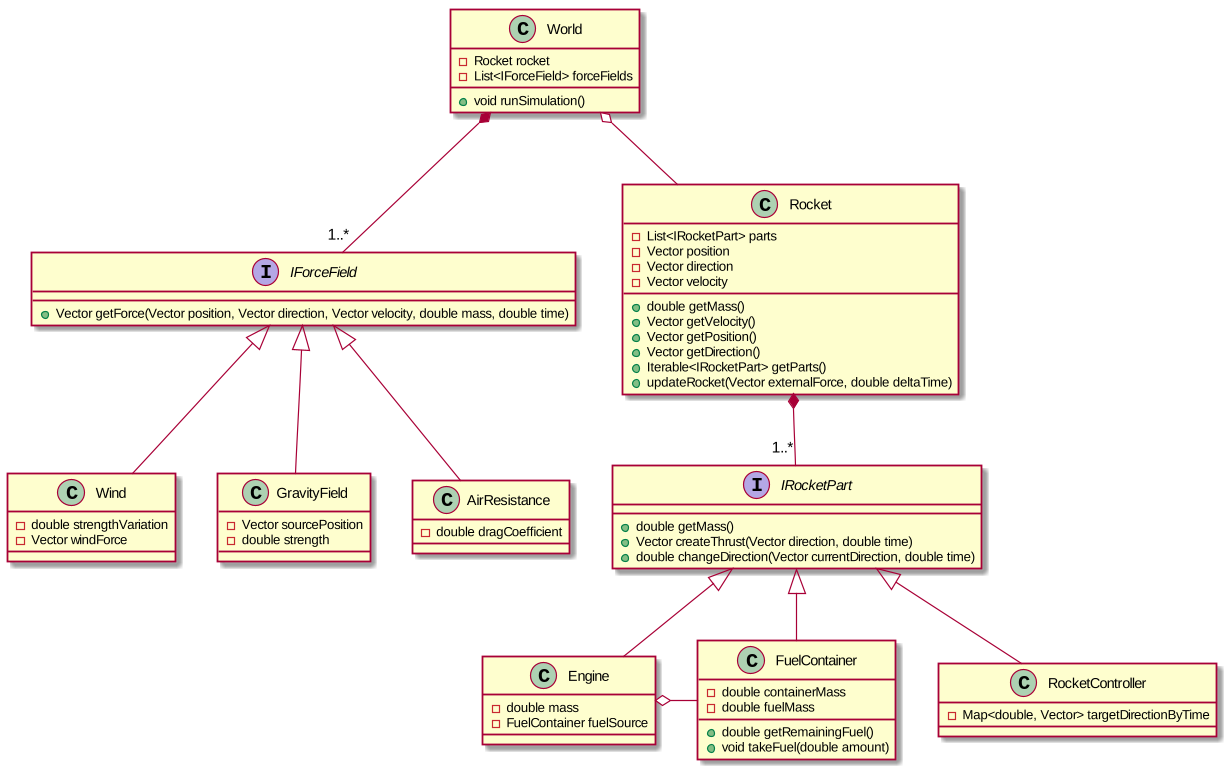
\includegraphics[width=17cm]{uml_diagram.png}

\end{document}
